\section{Stima dei costi}
\label{sec:stima_costi}

\par Alla luce delle analisi sulla natura del capitolato ChatSQL e sui rischi che potrebbero insorgere nell'arco del progetto, il team ha stilato una stima preliminare dei costi. Il preventivo viene rivalutato e, se necessario, aggiornato migliorativamente alla fine di ogni \glossario{sprint}.

\subsection{Ultimo aggiornamento: 2024-06-05}

\begin{minipage}{\textwidth}
\begin{table}[H]
  \begin{adjustwidth}{-0.5cm}{-0.5cm}
    \centering
    \begin{tabular}{|P{2.9cm}|P{2.4cm}|P{2.4cm}|P{2.4cm}|>{\arraybackslash}P{2.4cm}|}
    \hline
    \textbf{Ruoli} & \textbf{Ore per ruolo} & \textbf{Ore individuali} & \textbf{Costo orario (in \texteuro)} & \textbf{Costo totale (in \texteuro)} \\
    \hline
    \Responsabile[U]{} & 63 & 9 & 30,00 & 1.890,00 \\ 
    \hline
    \Amministratore[U]{} & 71 & 10 & 20,00 & 1.420,00 \\ 
    \hline
    \Analista[U]{} & 63 & 9 & 25,00 & 1.575,00 \\ 
    \hline
    \Progettista[U]{} & 140 & 20 & 25,00 & 3.500,00 \\ 
    \hline
    \Programmatore[U]{} & 162 & 23 & 15,00 & 2.430,00 \\ 
    \hline
    \Verificatore[U]{} & 147 & 21 & 15,00 & 2.205,00 \\ 
    \hline
    Totale & 646 & 92 & / & 13.020,00 \\ 
    \hline
  \end{tabular}
  \caption{Stima dei costi - ultimo aggiornamento: 2024-06-05}\label{tab:stima-costi}
  \end{adjustwidth}
\end{table}
\end{minipage}

\begin{figure}[H]
  \centering
  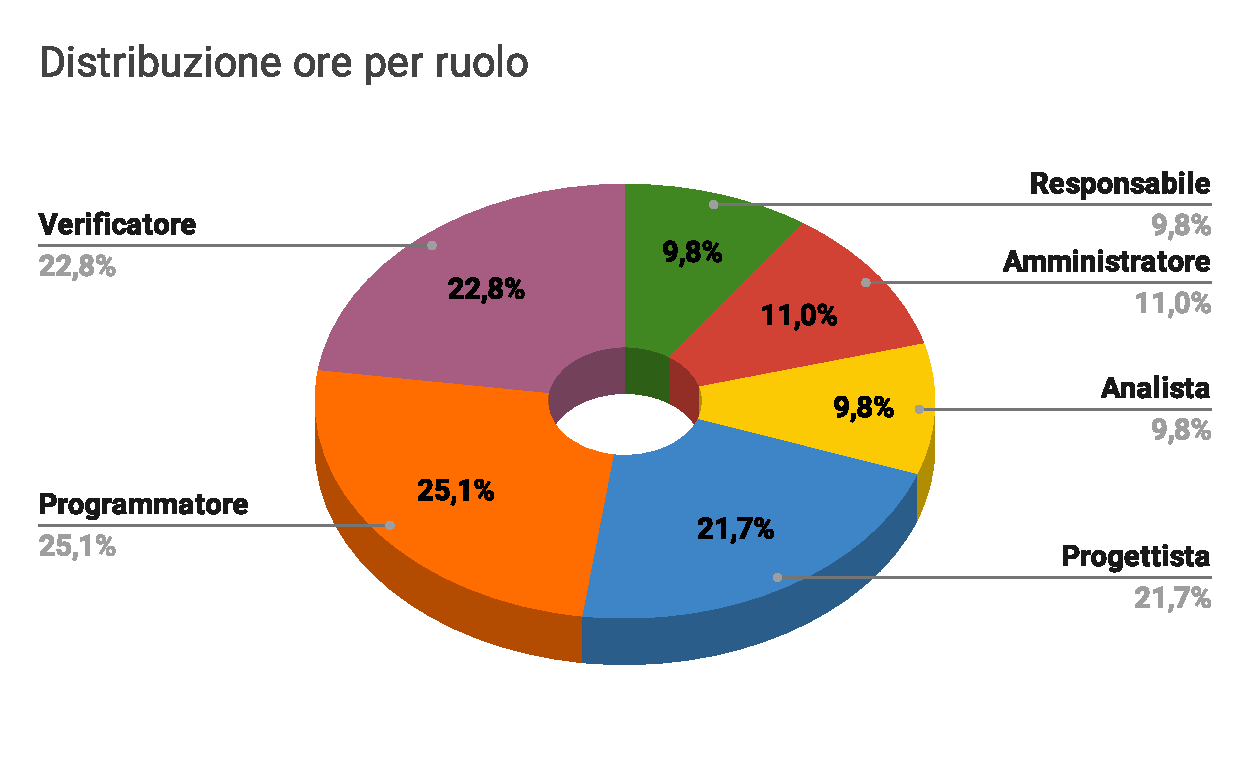
\includegraphics[width=0.90\textwidth]{assets/Preventivo/Totale/distribuzione_ore_ruolo.pdf}
  \caption{Distribuzione oraria per ruolo - ultimo aggiornamento: 2024-06-05}
\end{figure}

\subsection{Preventivo "a finire"}\label{sec:preventivo-a-finire}
\subsubsection{Ultimo aggiornamento: 2024-09-20}

\begin{minipage}{\textwidth}
Di seguito è riportato il preventivo "a finire", soggetto a miglioramento continuo in base alle considerazioni del consuntivo di periodo.
\begin{table}[H]
  \centering
  \begin{adjustbox}{max width=\textwidth}
  \begin{tabular}{|c|c|c|c|c|c|c|c|}
    \hline
    \multicolumn{8}{|c|}{\textbf{Preventivo "a finire"}} \\
    \hline
    \textbf{Membro del team} & \textbf{Re} & \textbf{Am} & \textbf{An} & \textbf{Pt} & \textbf{Pr} & \textbf{Ve} & \textbf{Totale per persona} \\
    \hline
    Riccardo Cavalli & 0 & 0 & 0 & 0 & 0 & 0 & 0 \\
    \hline
    Raul Pianon & 0 & 0 & 0 & 0 & 0 & 0 & 0 \\
    \hline
    Martina Dall'Amico & 0 & 0 & 0 & 0 & 0 & 0 & 0 \\
    \hline
    Marco Cristo & 0 & 0 & 0 & 0 & 0 & 0 & 0 \\
    \hline
    Sebastiano Lewental & 0 & 0 & 0 & 0 & 0 & 0 & 0 \\
    \hline
    Mattia Zecchinato & 0 & 0 & 0 & 0 & 0 & 0 & 0 \\
    \hline
    Tommaso Stocco & 0 & 0 & 0 & 0 & 0 & 0 & 0 \\
    \hline
    \textbf{Totale per ruolo} & 0 & 0 & 0 & 0 & 0 & 0 & \textbf{0} \\
    \hline
    \textbf{Costo totale (in €)} & 0,00 & 60,00 & 0,00 & 0,00 & 0,00 & 0,00 & \textbf{0,00} \\
    \hline
  \end{tabular}
  \end{adjustbox}
  \caption{Preventivo "a finire" - ultimo aggiornamento: 2024-09-20}\label{tab:preventivo-a-finire}
\end{table}
\end{minipage}


\subsection{Consuntivo finale}\label{sec:consuntivo-finale}

\begin{minipage}{\textwidth}
Di seguito è riportato il consuntivo finale delle ore produttive di ciascun membro.
\begin{table}[H]
  \centering
  \begin{adjustbox}{max width=\textwidth}
  \begin{tabular}{|c|c|}
    \hline
    \multicolumn{2}{|c|}{\textbf{Consuntivo orario}} \\
    \hline
    \textbf{Membro del team} & \textbf{Ore produttive} \\
    \hline
    Riccardo Cavalli & 92 \\
    \hline
    Raul Pianon & 92 \\
    \hline
    Martina Dall'Amico & 92 \\
    \hline
    Marco Cristo & 92 \\
    \hline
    Sebastiano Lewental & 92 \\
    \hline
    Mattia Zecchinato & 92 \\
    \hline
    Tommaso Stocco & 92 \\
    \hline
    \textbf{Totale} & 644 \\
    \hline
  \end{tabular}
  \end{adjustbox}
  \caption{Consuntivo finale}\label{tab:consuntivo-finale}
\end{table}
\end{minipage}
